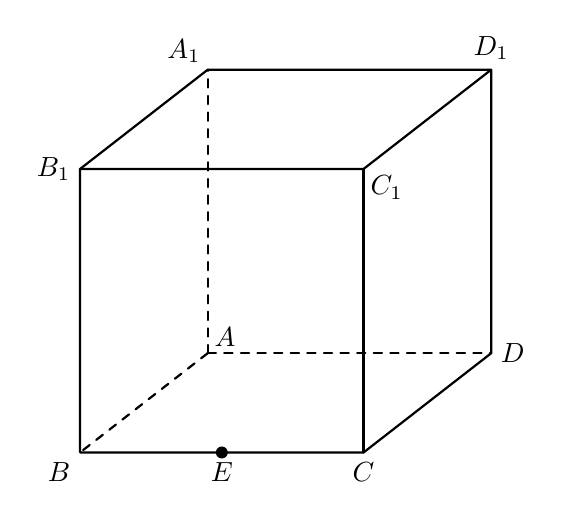
\begin{tikzpicture}[scale=1.8, line join=round, line cap=round, >=stealth]
  % 顶点坐标设定（正方体斜二测标准投影）
  \coordinate (B) at (0, 0);
  \coordinate (C) at (2.0, 0);
  \coordinate (A) at (0.9, 0.7);
  \coordinate (D) at (2.9, 0.7);

  \coordinate (B1) at (0, 2.0);
  \coordinate (C1) at (2.0, 2.0);
  \coordinate (A1) at (0.9, 2.7);
  \coordinate (D1) at (2.9, 2.7);

  % 棱 BC 中点 E
  \coordinate (E) at (1.0, 0);

  % 虚线部分（后侧与内部不可见棱）
  \draw[dashed, thick] (A) -- (B);
  \draw[dashed, thick] (A) -- (D);
  \draw[dashed, thick] (A) -- (A1);

  % 实线部分（外轮廓与可见棱）
  \draw[thick] (B) -- (C) -- (D) -- (D1) -- (A1) -- (B1) -- cycle;
  \draw[thick] (B1) -- (C1) -- (D1);
  \draw[thick] (C) -- (C1);

  % 关键点标记
  \fill (E) circle (1.2pt);

  % 顶点标注
  \node[below left] at (B) {$B$};
  \node[below] at (C) {$C$};
  \node[right] at (D) {$D$};
  \node[above right=-1pt] at (A) {$A$};

  \node[left] at (B1) {$B_1$};
  \node[below right=-1pt] at (C1) {$C_1$};
  \node[above] at (D1) {$D_1$};
  \node[above left=-1pt] at (A1) {$A_1$};

  \node[below] at (E) {$E$};
\end{tikzpicture}
